%
% 1-motivation.tex
%
% (c) 2023 Prof Dr Andreas Müller
%
\section{Vergleich von Funktionen
\label{buch:einleitung:section:vergleich}}
\kopfrechts{Vergleich von Funktionen}
Harmonische Analysis ist eine Methode, Funktionen in besser
verstandene Komponenten zu zerlegen.
Die Basis dafür ist die Möglichkeit, die ``Ähnlichkeit'' zwischen
Funktionen zu messen.
In diesem Abschnitt soll gezeigt werden, wie diese Idee der
``Ähnlichkeit'' sich natürlich in verschiedenen bekannten
Anwendungen ergibt.
Das Ziel ist, den Weg zum abstrakten Konzept des verallgemeinerten
Skalarproduktes aufzuzeigen.
\index{Skalarprodukt}%

%
% Kovarianz als Mass der Ähnlichkeit von Datenreihen
%
\subsection{Kovarianz als Mass der Ähnlichkeit von Datenreihen}
In der Statistik lernt man, dass Beziehungen zwischen Zufallsvariablen
\index{Zufallsvariable}%
$X$ und $Y$ durch die Kovarianz gemessen werden.
\index{Kovarianz}%
Wir nehmen für die folgende Diskussion der Einfachheit halber an,
dass die Erwartungswerte $E(X)=E(Y)=0$ sind.
\index{Erwartungswert}%
In diesem Fall ist die Kovarianz der Erwartungswert $E(XY)$ des
Produkts der beiden Zufallsvariablen.
Für Stichproben $x_i$ und $y_i$, $i=1,\dots,n$, kann die Kovarianz mit
Hilfe der empirischen Kovarianz
\[
\operatorname{cov}(X,Y)
=
\frac{1}{n}
\sum_{i=1}^n x_iy_i
\]
geschätzt werden.
Abbildung~\ref{buch:einleitung:fig:kovvergleich} zeigt Beispiele
verschiedener Stichproben mit mehr oder weniger grosser
Kovarianz.
Im rechten Teil der Abbildung sind die Paare $(x_i,y_i)$ als
Punktepaare aufgezeichnet.

\begin{figure}
\begin{center}
\begin{tikzpicture}[>=latex,thick]
%\draw (-7,-15.8) rectangle (7,2.7);
\clip (-7,-15.8) rectangle (7,2.7);
\begin{scope}
\node at (0,0) {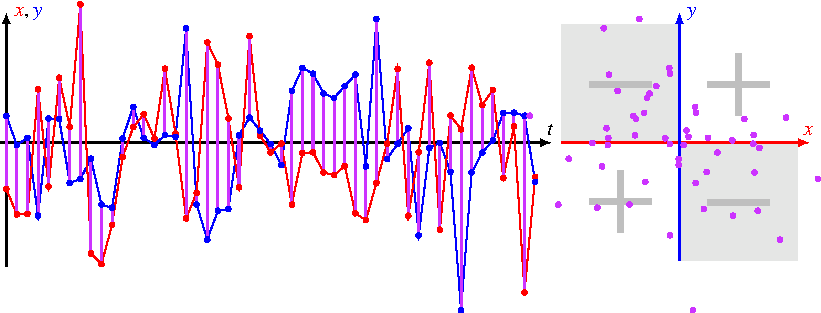
\includegraphics{chapters/000-einleitung/images/randrand.pdf}};
\end{scope}
\begin{scope}[yshift=-4.5cm]
\node at (0,0) {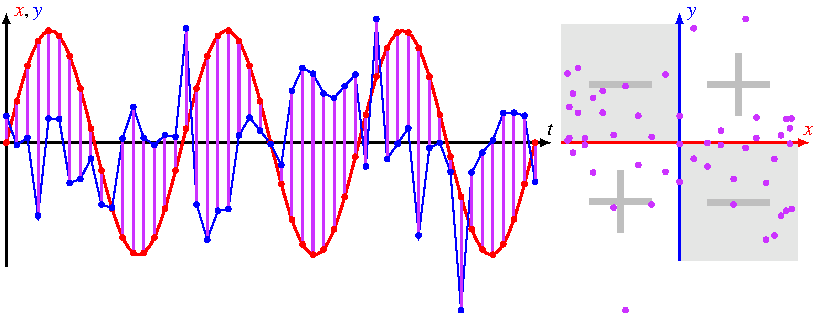
\includegraphics{chapters/000-einleitung/images/sinrand.pdf}};
\end{scope}
\begin{scope}[yshift=-9.0cm]
\node at (0,0) {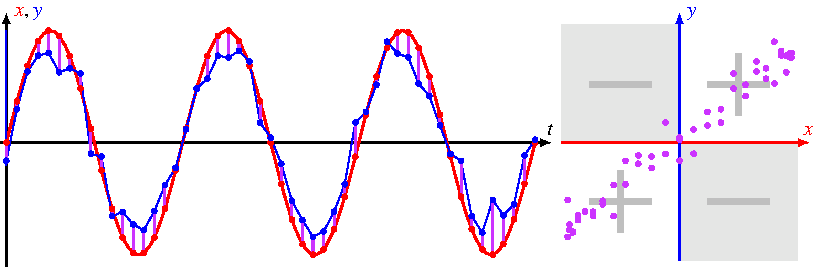
\includegraphics{chapters/000-einleitung/images/sinsin.pdf}};
\end{scope}
\begin{scope}[yshift=-13.5cm]
\node at (0,0) {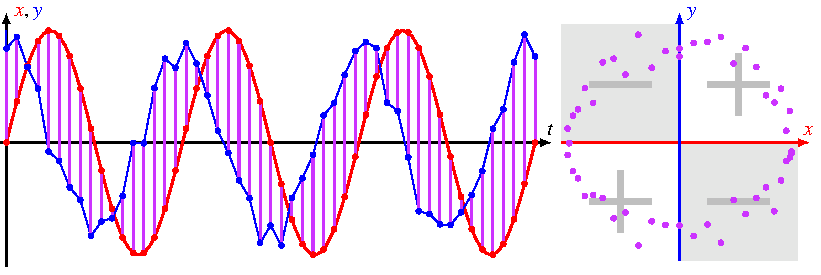
\includegraphics{chapters/000-einleitung/images/sincos.pdf}};
\end{scope}
\end{tikzpicture}
\end{center}
\caption{Stichproben verschiedener Zufallsvariablen mit unterschiedlich
ausgeprägter Kovarianz
\label{buch:einleitung:fig:kovvergleich}}
\end{figure}


Zuoberst in der Abbildung~\ref{buch:einleitung:fig:kovvergleich}
sind zwei ganz zufällige Zahlenreihen dargestellt.
Die Vorzeichen der Produkte $x_iy_i$ sind wild gemischt, die Punkte
verteilen sich gleichmässig über alle vier Quadranten.
Im Mittel heben sich die Beiträge der Produkte $x_iy_i$ weg, die
Kovarianz ist sehr klein.

In der zweiten Graphik ist die rote Zahlenreihe durch eine Sinusfunktion
ersetzt worden.
\index{Sinusfunktion}%
Die $x$-Koordinaten der Punkte sind jetzt nicht mehr zufällig, die
$y$-Koordinaten sind aber immer noch ungeordnet. 
Auch in diesem Fall sind die Punkte gleichmässig über alle Quadranten
verteilt und die Kovarianz ist klein.

In der dritten Graphik sind die blauen Punkte Werte einer
Sinusfunktion, denen kleine zufällige Fehler überlagert sind.
Die Punkte $(x_i,y_i)$ sind jetzt nicht mehr zufällig verteilt,
sie bewegen sich entlang der $45^\circ$-Geraden im ersten
und dritten Quadranten.
Für die meisten Punkte ist das Produkt $x_iy_i$ daher positiv und
die Kovarianz, die Summe dieser Produkte, wird gross.
Die zufällig gestörte blaue Sinusfunktion ist der exakten roten
Sinusfunktion ziemlich ähnlich.

In der letzten Graphik schliesslich werden eine Sinusfunktion und
\index{Cosinusfunktion}%
eine mit zufälligen Abweichungen gestörte Cosinusfunktion miteinenader
verglichen.
Zwar gibt es jetzt einen klaren Zusammenhang, aber die Punkte sind
wieder über alle vier Quadranten verteilt.
Die Kovarianz ist wieder klein.
Tatsächlich ist die gestörte Cosinusfunktion eben nicht ähnlich zu 
einer Sinusfunktion, sondern zu einer Cosinusfunktion.

Die Kovarianz kann also dazu verwendet werden, eine unbekannten
Datenreihe mit verschiedenen Funktionen zu vergleichen und zu
beurteilen, welche am ``ähnlichsten'' ist.

\subsubsection{Zufallsvariablen mit Erwartungswert $\ne  0$}
Für Zufallsvariablen, deren Erwartungswerte nicht verschwinden,
wird die Formel für die Kovarianz etwas komplizierter, sie lautet
\begin{equation}
\operatorname{cov}(X,Y) = E(XY) - E(X)E(Y).
\label{buch:einleitung:eqn:cov}
\end{equation}
Doch dies ändert nichts an der Ähnlichkeit der Kovarianz 
mit einem Skalarprodukt.

Dazu muss man allerdings berücksichtigen, dass zwei Zufallsvariablen
im Vergleich zu den Schwankungen sehr grosse Erwartungswerte haben können.
Dies hat zur Folge, dass $E(XY)$ von den Erwartungswerten dominiert
wird, die Schwankungen spielen nur eine untergeordnete Rolle.

Die Zufallsvariable $X-E(X)$ hat wegen
$E(X-E(X))=E(X)-E(E(X))=E(X)-E(X)=0$ Erwartungswert $0$.
Für Datenreihen $x_i$ und $y_i$ bedeutet dies, dass man
die Koordinaten $x$ und $y$ durch neue Koordinaten ersetzt,
so dass die Punktwolke aus den Punkten $(x_i,y_i)$ den
Nullpunkt des Koordinatensystems als Schwerpunkt hat.
Der Erwartungswert des Produktes von $X-E(X)$ und $Y-E(Y)$
ist dann
\begin{align*}
E(\, (X-E(X))\cdot(Y-E(Y))\, )
&=
E(XY)-E(X\cdot E(Y)) - E(E(X)\cdot Y) + E(E(X)E(Y))
\\
&=
E(XY) - E(X)E(Y)-E(X)E(Y)+E(X)E(Y)
\\
&=
E(XY)-E(X)E(Y),
\end{align*}
dies ist die allgemeine Definition~\eqref{buch:einleitung:eqn:cov}
der Kovarianz.

%
% Das Skalarprodukt in der Vektorgeometrie
%
\subsection{Das Skalarprodukt in der Vektorgeometrie}
Das Skalarprodukt wird in einem rechtwinkligen Koordinatensystem nach der
\index{Skalarprodukt}
Formel
\begin{equation}
\vec{x}\cdot\vec{y} = x_1y_1 + x_2y_2 + x_3y_3 = \sum_{i=1} x_iy_i
\label{buch:einleitung:motiviation:equn:vektorskalar}
\end{equation}
berechnet.
Es verschwindet, wenn die Vektoren $\vec{x}$ und $\vec{y}$ orthogonal
sind, man könnte sagen,
wenn die Vektoren so verschiedene Richtung wie möglich haben.
Die Orthogonalprojektion von $\vec{x}$ auf die Richtung $\vec{y}$,
\index{Orthogonalprojektion}%
auch die Komponente von $\vec{x}$ in der Richtung von $\vec{y}$ genannt,
hat die Länge 
\[
\frac{\vec{x}\cdot\vec{y}}{|\vec{y}|}
=
\vec{x}\cdot \vec{y}^0.
\]
Das Skalarprodukt zweier Vektoren ist nicht grösser als das Produkt
der Vektorlängen.
Die Cauchy-Schwarz-Ungleichung, ausführlich diskutiert in
\index{Cauchy-Schwarz-Ungleichung}%
Abschnitt~\ref{buch:skalarprodukte:section:cauchyschwarz},
zeigt, dass das Skalarprodukt mit dem Produkt der Vektorlängen
genau dann übereinstimmt, wenn die Vektoren die gleiche Richtung
haben, wenn sie also linear abhängig sind.
Die Berechnungsformel~\eqref{buch:einleitung:motiviation:equn:vektorskalar}
deckt sich mit der Formel zur Berechnung der empirischen Kovarianz.

%
% Skalarprodukte von Funktionen
%
\subsection{Skalarprodukte von Funktionen}
Die bisherigen Ausführungen zeigen, dass ein Skalarprodukt von
Vektoren in $\mathbb{R}^n$ als ein Mass für die Ähnlichkeit von Vektoren
dienen kann. 
Die Koordinaten eines Vektors in einer orthogonalen Basis werden
als Skalarprodukte des Vektors mit den Basisvektoren bestimmt.
Die Koordinaten geben an, wie ``ähnlich'' zu den Basisvektoren ein Vektor
ist.
Die Linearkombination der orthonormierten Basisvektoren $b_i$ mit den
Koeffizienten $(x\cdot b_i)$ ergibt wieder den Vektor 
\[
x = \sum_{i=1}^n (b_i\cdot x) \, b_i.
\]
Das Skalarprodukt ist also eine besonders effiziente und natürlich
Methode, einen Vektor in Komponenten parallel zu den Basisvektoren
zu zerlegen und den Vektor auch wieder aus den Basisvektoren zu
synthetisieren.

Diese Idee kann auf sehr viele weitere Situation ausgedehnt werden,
wenn sich das Konzept des Skalarproduktes darauf übertragen lässt.
Aus der linearen Algebra \cite{buch:linalg} weiss man, dass sich
aus den Axiomen eines 
Skalarproduktes und aus einer Basis alles konstruieren lässt, was
man für eine solche Analyse benötigt.
Funktionen bilden bereits einen Vektorraum.
\index{Vektorraum}%
Wenn es also gelingt,
ein Skalarprodukt zu konstruieren, dann kann man damit beginnen,
orthonormierte Basen zur Analyse von Funktionen zu verwenden.

%
% Interessante Basen
%
\subsection{Interessante Basen}
Der Gram-Schmidt-Algorithmus zur Konstruktion einer orthonormierten
\index{Gram-Schmidt-Algorithmus}%
Basis zeigt, dass sich ausgehend von jeder beliebigen linear
unabhängigen Funktionenmenge eine Basis konstruieren lässt.
Zum Beispiel kann man orthonormierte Basen aus Polynomen konstruieren.
Da Polynome sehr leicht zu evaluieren sind, ergeben sich für die
Numerik nützliche Funktionsbasen.
\index{Numerik}%

Meistens haben die Funktionen, die man analysierte möchte, noch
viel mehr Struktur.
Joseph Fourier hat beobachtet, dass periodische Funktionen zu einer
\index{Fourier, Joseph Baptiste}%
besonders erfolgreichen Theorie führen.
Man kann seine Basisfunktion dadurch charakterisieren, dass sie
unter Translation des Arguments invariant sind.
Verlangt man ausserdem Differenzierbarkeit, dann sind die
Fourier-Basisfunktionen Eigenfunktionen des Ableitungsoperators.
\index{Fourier-Basisfunktionen}%
\index{Eigenfunktionen}%
\index{Ableitungsoperator}%

Tatsächlich treten orthogonale Funktionensystem im Zusammenhang
mit partiellen Differentialgleichungen auf ganz natürliche Art auf.
Ist $L$ ein selbstadjungierter Operator, dann sind die Eigenfunktionen
dieses Operators orthogonal.
Die trigonometrischen Funktionen sind zum Beispiel Eigenfunktionen
des Operators der zweiten Ableitung, ausserdem ist die zweite
Ableitung selbstadjungiert im Raum der periodischen Funktionen
mit dem $L^2$-Skalarprodukt.
Der Laplace-Operator hat ähnliche Eigenschaften und führt
auf verallgemeinerte harmonische Analysis für Funktionen auf
einer grossen Zahl von Definitionsgebieten, die auch für
Anwendungen wichtig sind.

Die Fourier-Funktionen haben aber noch weitere wichtige Eigenschaften.
Das Definitionsgebiet hat die Struktur einer Gruppe, was sich zum
\index{Gruppe}%
Beispiel in den Additionstheoremen äussert.
Daraus lässt sich eine weitere Operation konstruieren, die Faltung.
\index{Faltung}%
Es zeigt sich, dass die Verwendung der Fourier-Basis auch dazu führt,
dass die Fourier-Transformation aus einem Faltungsprodukt ein gewöhnliches
\index{Fourier-Transformation}%
Produkt der Fourierkoeffizienten macht.
Auch diese Eigenschaft lässt sich auf eine grosse Zahl weiterer
Gruppen auf interessante Art verallgemeinern.

Es gibt also verschiedene Möglichkeiten, ein Funktionsystem so
zu wählen, dass es einerseits optimal an eine Aufgabenstellung
angepasst ist, andererseits aber eine Analyse mit einem Skalarprodukt
und Synthese ermöglicht.
Das Ziel dieses Seminars ist, diese Möglichkeiten auszuloten
und einige wichtige Anwendungen zu illustrieren.




